% Copyright 2026 Sreeram Anil
% SPDX-License-Identifier: CC-BY-4.0
% =============================================================================
%  Fuzzy-logic adaptive Kalman filter (Mamdani covariance tuning)
% =============================================================================
\chapter{Fuzzy-logic adaptive Kalman filter (Fuzzy-AKF)}
\label{ch:fuzzyakf}

\section*{At a glance}
\begin{tabular}{@{}l>{\raggedright\arraybackslash}p{0.76\textwidth}@{}}
Family & Adaptive Kalman \\
Header & \texttt{include/estkit/filters/fuzzy\_akf.hpp} \\
Registered name & \texttt{Fuzzy-AKF} \\
State dimension & $n_x = 4$ (cell model) --- generic in $n_x, n_u, n_y$; window $N$ and grid $N_g$ are template parameters \\
Cost per step & EKF $+\,\mathcal{O}(n_y^2) + 3N_g$ flops; $\approx 730$\,ns/step, $N n_y$ reals of buffer, no heap \\
Primary references & \cite{loebis2004fuzzy,mamdani1975,zadeh1965,mohamed1999adaptive,jwo2007fuzzy} \\
\end{tabular}

\section{Motivation and aerospace/BMS relevance}
The covariance-matching estimators of \cref{ch:iaeakf} compute $\hat{\mR}$ in closed form and apply
it immediately.  That is statistically efficient but operationally brittle: the estimate inherits
the full variance of a short window, it can jump by an order of magnitude between consecutive
samples, and it has no notion of "how sure am I that something changed".  Engineers who have to
certify a filter frequently prefer a \emph{supervisor} that changes the tuning gradually, in a way
that can be stated in words and drawn on one page: "if the residuals are much larger than expected,
increase the assumed measurement noise a little; if they are much smaller, decrease it a little;
otherwise do nothing".

That is precisely a fuzzy inference system in the sense of Zadeh \cite{zadeh1965} and Mamdani
\cite{mamdani1975}.  Loebis, Sutton, Chudley and Naeem \cite{loebis2004fuzzy} applied it to the
navigation filter of an autonomous underwater vehicle: they form a scalar \emph{degree of matching}
(DoM) between the measured and the theoretical innovation covariance, feed it to a small rule base
with triangular membership functions, and use the defuzzified output to retune $\mR$ (and, in a
second loop, $\mQ$).  The same construction has since been combined with the strong tracking filter
for GPS navigation \cite{jwo2007fuzzy}.

The engineering value in a BMS is the rate limit.  A cell-voltage channel can be hit by a
\SI{50}{\milli\volt} spike from a single corrupted SPI frame; a closed-form estimator will respond
to the resulting window average with a step change in the gain, whereas a rate-limited fuzzy
supervisor slews the tuning smoothly and cannot be driven to an extreme by a short burst.  The price
is a slower response to a genuine change, and the whole design of this chapter is about where that
trade sits.

\section{Problem statement and assumptions}
The plant is \eqref{eq:sh:proc}--\eqref{eq:sh:meas}.  The filter carries a scalar
\emph{measurement-noise scaling} $s_k>0$ and uses
\begin{equation}
\hat{\mR}_k = s_k\,\mR(\xminus_k,\vu_k)
\label{eq:fz:R}
\end{equation}
in place of the nominal model covariance.  The design problem is to drive $s_k$ from the innovation
sequence.  We assume, as in \cref{ch:iaeakf}, that the innovations are approximately white
(\cref{as:iae:white}) and that the statistics are stationary over the window
(\cref{as:iae:stat}).

\section{Derivation}

\subsection{The degree of matching}
Let $\bm{e}_j=\vy_j-h(\xminus_j,\vu_j)$ and form the windowed sample covariance
\begin{equation}
\hat{\mC}_k = \frac{1}{N}\sum_{j=k-N+1}^{k}\bm{e}_j\bm{e}_j^\T
\label{eq:fz:C}
\end{equation}
and the filter's own prediction of it,
$\mS_k = \mH_k\Pminus_k\mH_k^\T + \hat{\mR}_{k-1}$.  Loebis et al.\ compare the two; the
dimensionless comparison used here is
\begin{equation}
\boxed{\;\mathrm{DoM}_k = \frac{\tr\hat{\mC}_k - \tr\mS_k}{\tr\mS_k}\;}
\label{eq:fz:dom}
\end{equation}
so that $\mathrm{DoM}_k=0$ means perfect matching, $\mathrm{DoM}_k>0$ means the filter is
over-confident (residuals larger than predicted) and $\mathrm{DoM}_k<0$ means it is
under-confident.  Normalising by $\tr\mS_k$ rather than using the raw difference makes the input
scale-free, so the same rule base and the same membership functions work for any measurement unit
and any operating point --- essential for a generic filter.

\subsection{The rule base}
Three membership functions partition the DoM universe.  With the normalised input
$d = \mathrm{DoM}_k/c$, where $c$ is the design constant \texttt{dom\_scale},
\begin{equation}
\mu_{\mathsf N}(d) = \begin{cases}1,& d\le-1\\ -d,& -1<d<0\\ 0,& d\ge0\end{cases}
\qquad
\mu_{\mathsf Z}(d) = \begin{cases}1-|d|,& |d|<1\\ 0,&\text{else}\end{cases}
\qquad
\mu_{\mathsf P}(d) = \begin{cases}0,& d\le0\\ d,& 0<d<1\\ 1,& d\ge1 .\end{cases}
\label{eq:fz:mf}
\end{equation}
The outer two are shoulders, so $\mu_{\mathsf N}+\mu_{\mathsf Z}+\mu_{\mathsf P}=1$ for every $d$
(a \emph{partition of unity}): at most two rules fire, the firing strengths are already normalised,
and the inference is continuous and piecewise linear in $d$.  The rule base is
\begin{center}
\begin{tabular}{@{}lll@{}}
\toprule
& antecedent & consequent \\
\midrule
$\mathsf{R}_1$ & IF $\mathrm{DoM}$ is $\mathsf N$ (negative) & THEN $\Delta$ is $\mathsf D$ (decrease $s$) \\
$\mathsf{R}_2$ & IF $\mathrm{DoM}$ is $\mathsf Z$ (zero)     & THEN $\Delta$ is $\mathsf H$ (hold $s$) \\
$\mathsf{R}_3$ & IF $\mathrm{DoM}$ is $\mathsf P$ (positive) & THEN $\Delta$ is $\mathsf I$ (increase $s$) \\
\bottomrule
\end{tabular}
\end{center}
with consequent membership functions that are unit-half-width triangles on the normalised output
axis $v\in[-1.5,1.5]$, centred at $c_1=-1$, $c_2=0$, $c_3=+1$:
$\mathrm{tri}_r(v)=\max(0,\,1-|v-c_r|)$.

\subsection{Mamdani inference and centroid defuzzification}
Mamdani's min-implication clips each consequent at its rule's firing strength
$w_r$, and max-aggregation takes the pointwise maximum:
\begin{equation}
\mu^{\text{agg}}(v) = \max_{r\in\{1,2,3\}}\ \min\!\big(w_r,\ \mathrm{tri}_r(v)\big),
\qquad w_1=\mu_{\mathsf N}(d),\ w_2=\mu_{\mathsf Z}(d),\ w_3=\mu_{\mathsf P}(d).
\label{eq:fz:agg}
\end{equation}
The crisp output is the centre of area of the aggregated set,
\begin{equation}
v^\star = \frac{\int v\,\mu^{\text{agg}}(v)\,\mathrm{d}v}{\int \mu^{\text{agg}}(v)\,\mathrm{d}v}
\;\approx\; \frac{\sum_{g=1}^{N_g} v_g\,\mu^{\text{agg}}(v_g)}{\sum_{g=1}^{N_g}\mu^{\text{agg}}(v_g)},
\qquad v_g = -1.5 + 3\frac{g-1}{N_g-1},
\label{eq:fz:centroid}
\end{equation}
evaluated on a fixed grid of $N_g$ points.  The grid is what makes this a genuine Mamdani centroid
rather than the weighted-average (Sugeno) short cut; it costs $3N_g$ multiply--adds per sample,
$123$ for the default $N_g=41$, which is small next to the EKF's $\approx500$ flops.

\subsection{The tuning law and its fixed point}
The defuzzified output is interpreted as an increment of $\ln s$:
\begin{equation}
s_k = \mathrm{clamp}\Big(s_{k-1}\exp\big(\delta\, v^\star\big),\ s_{\min},\ s_{\max}\Big),
\label{eq:fz:law}
\end{equation}
where $\delta = \texttt{opts.step}$ is the maximum change of $\ln s$ per sample, i.e.\ a
\emph{rate limit}.  Working in the logarithm makes the law scale-invariant (a factor-of-ten error is
corrected in the same number of samples whether $s$ is $1$ or $100$) and guarantees $s_k>0$.

The fixed point of \eqref{eq:fz:law} is $v^\star=0$, which by \eqref{eq:fz:mf} requires
$\mathrm{DoM}_k=0$, i.e.\ $\tr\mS_k=\tr\hat{\mC}_k$; writing this out,
\begin{equation}
s^\star\,\tr\mR = \tr\hat{\mC}_k - \tr\big(\mH_k\Pminus_k\mH_k^\T\big),
\label{eq:fz:fp}
\end{equation}
which is \emph{exactly} the IAE estimator \eqref{eq:iae:R} in trace form.  The fuzzy supervisor is
therefore a rate-limited, smoothed realisation of innovation-based adaptive estimation: it converges
to the same answer, but it slews there at no more than $\delta$ nepers per sample and it cannot be
displaced from it by a short burst of large innovations.  Stating the fixed point explicitly is what
turns a heuristic into an analysable controller --- and it immediately gives the design rule for
$\delta$: the time to correct a factor-$\kappa$ error in $s$ is $\ln\kappa/\delta$ samples.

\section{Algorithm}
\begin{algorithm}[H]
\caption{Fuzzy-AKF --- one sampling period}
\begin{algorithmic}[1]
\Require $\xplus_{k-1},\Pplus_{k-1},\vu_{k-1},\vy_k,\vu_k,s_{k-1}$, ring buffer and running sum $\Sigma$
\State \textbf{Time update:} $\xminus_k\gets f(\xplus_{k-1},\vu_{k-1})$;\quad $\Pminus_k\gets\mF\Pplus_{k-1}\mF^\T+\mQ_k$
\State \textbf{Innovation:} $\mH\gets\partial h/\partial\vx|_{\xminus_k}$;\quad $\bm{e}_k\gets\vy_k-h(\xminus_k,\vu_k)$
\State \textbf{Window:} slide the ring buffer, $\Sigma\gets\Sigma-\bm{e}_{k-N}\bm{e}_{k-N}^\T+\bm{e}_k\bm{e}_k^\T$;\quad $\hat{\mC}_k\gets\Sigma/n$
\If{$n\ge N_{\min}$}
  \State $\mS\gets\mH\Pminus_k\mH^\T+s_{k-1}\mR_k$;\quad $\mathrm{DoM}\gets(\tr\hat{\mC}_k-\tr\mS)/\tr\mS$
  \State $d\gets\mathrm{clamp}(\mathrm{DoM}/c,-2,2)$;\quad evaluate $w_{1,2,3}$ from \eqref{eq:fz:mf}
  \State $v^\star\gets$ centroid of $\max_r\min(w_r,\mathrm{tri}_r(\cdot))$ on the $N_g$-point grid
  \State $s_k\gets\mathrm{clamp}(s_{k-1}e^{\delta v^\star},s_{\min},s_{\max})$
\EndIf
\State $\hat{\mR}_k\gets s_k\mR_k$
\State \textbf{Gain and update:} $\mS_k\gets\mH\Pminus_k\mH^\T+\hat{\mR}_k$;\quad $\mK_k\gets\Pminus_k\mH^\T\mS_k\inv$;\quad
       $\xplus_k\gets\xminus_k+\mK_k\bm{e}_k$;\quad Joseph update of $\Pplus_k$
\State \textbf{Constrain:} $\xplus_k\gets\mathrm{constrain}(\xplus_k)$
\Ensure $\xplus_k,\Pplus_k,s_k$
\end{algorithmic}
\end{algorithm}

\section{Application to the battery model}
With $n_y=1$ the traces in \eqref{eq:fz:dom} are scalars and
$\mathrm{DoM}_k = (\hat C_k - S_k)/S_k$ with $\hat C_k$ the mean squared voltage innovation over the
window.  Options used in the benchmark: $N=50$ samples ($=\SI{5}{\second}$, the window length used
by Loebis et al.\ scaled to this sample rate), $N_g=41$ grid points, $c=0.5$ (a $50\,\%$ covariance
mismatch saturates the "negative"/"positive" membership), $\delta=0.3$, $s\in[0.2,\,2\times10^3]$.

The rate limit deserves a word.  $\delta=0.3$ per sample is $\SI{3}{\per\second}$ at
\SI{10}{\hertz}, so $s$ can change by a factor of $e^3\approx20$ per second and needs
$\ln(93)/0.3\approx15$ samples $=\SI{1.5}{\second}$ to cover the factor-$93$ change demanded by the
\texttt{noise\_step} scenario --- fast enough to be useful, slow enough that a single corrupted
sample (which moves the window mean by $1/N$ of its value) barely moves $s$.  Values
$\delta\in\{0.002,0.01,0.05,0.1,0.3\}$ were evaluated; below $\delta\approx0.1$ the supervisor is too
slow to correct the large mismatch of the \texttt{combined} scenario within the mission and the
filter never reaches the $2\,\%$ band, which is why the comparatively brisk $0.3$ was adopted.  The
saturation constant $c=0.5$ and the bounds were not found to be critical (the metrics change by
under $10\,\%$ over $c\in[0.2,2]$).

\section{Implementation notes}
\begin{itemize}[leftmargin=1.4em]
\item \textbf{Heap-free fuzzy engine.}  The membership functions are evaluated in closed form, the
      aggregation and centroid are computed on a compile-time-sized grid
      (\texttt{template<class Model,int NWIN,int NG>}), and the only transcendental call is a single
      guarded \texttt{exp} per sample.  No lookup tables, no dynamic memory, fully deterministic
      execution time --- the properties that make a fuzzy supervisor attractive on a safety-related
      MCU in the first place.
\item \textbf{Partition of unity.}  Because $\sum_r w_r = 1$ by construction, no normalisation of
      the firing strengths is needed and the denominator of \eqref{eq:fz:centroid} can never vanish
      (it is guarded anyway).
\item \textbf{Buffer.}  $N n_y$ reals ($400$\,bytes for the cell model) plus one running sum,
      updated in $\mathcal{O}(n_y^2)$.
\item \textbf{Cost.}  \SI{727}{\nano\second}/step against \SI{478}{\nano\second}/step for the EKF.
      The overhead is dominated by the $3N_g=123$ grid evaluations; dropping to $N_g=11$ or using
      Sugeno singletons would remove most of it at the cost of a slightly coarser centroid.
\item \textbf{float32.}  Metrics agree with the double build to three digits; no divergence.
\item \textbf{Limitations.}  Being a rate-limited IAE, it inherits IAE's inability to distinguish
      sensor noise from model error, and it adds a lag.  It also adapts only $\mR$; Loebis et al.\
      use a second fuzzy loop for $\mQ$, which is not implemented here for the identifiability
      reasons set out in \cref{ch:sagehusaakf}.
\end{itemize}

\section{Benchmark results}
% Copyright 2026 Sreeram Anil
% SPDX-License-Identifier: CC-BY-4.0
\begin{table}[H]\centering\footnotesize\setlength{\tabcolsep}{4pt}
\caption{Fuzzy-AKF: cell-level benchmark on the eVTOL mission (mean over seeds; RMSE and max error in \% SOC; $t_\mathrm{conv}$: first time the error stays below 2\,\% for 60\,s, -- = never; EKF reference: steady-state RMSE of the plain EKF on the same data).}\label{tab:cell_FuzzyAKF}
\begin{tabular}{llrrrrrcrr}\toprule
plant & scenario & RMSE & RMSE$_\mathrm{ss}$ & max & $t_\mathrm{conv}$ [s] & RMSE$_v$ [mV] & div. & EKF ref. & ns/step \\ \midrule
ECM & nominal & 0.19 & 0.05 & 1.15 & 0 & 0.79 & no & 0.05 & 727 \\
ECM & init\_error & 0.16 & 0.08 & 0.71 & 0 & 2.12 & no & 0.05 & 729 \\
ECM & current\_bias & 0.54 & 0.64 & 1.39 & 0 & 0.87 & no & 0.61 & 728 \\
ECM & noise\_step & 0.19 & 0.05 & 1.15 & 0 & 1.02 & no & 0.12 & 728 \\
ECM & outliers & 0.25 & 0.05 & 2.50 & 0 & 1.47 & no & 0.21 & 726 \\
ECM & cold & 0.20 & 0.20 & 1.17 & 0 & 1.89 & no & 0.16 & 725 \\
ECM & hot & 0.18 & 0.03 & 1.00 & 0 & 0.54 & no & 0.03 & 727 \\
ECM & aged\_cell & 1.04 & 1.25 & 2.62 & 0 & 22.45 & no & 1.52 & 725 \\
ECM & param\_mismatch & 0.83 & 0.96 & 1.91 & 0 & 6.12 & no & 1.36 & 723 \\
ECM & sensor\_dropout & 0.19 & 0.06 & 1.15 & 0 & 0.88 & no & 0.46 & 723 \\
ECM & preisach & 0.61 & 0.20 & 1.80 & 0 & 0.82 & no & 0.20 & 728 \\
ECM & combined & 5.67 & 2.56 & 14.93 & 1753 & 15.01 & no & 12.44 & 735 \\
\midrule
SPM & nominal & 3.11 & 3.18 & 3.80 & 0 & 1.53 & no & 3.73 & 698 \\
SPM & init\_error & 3.42 & 3.43 & 4.29 & 0 & 2.45 & no & 3.81 & 701 \\
SPM & current\_bias & 4.45 & 5.16 & 5.85 & 0 & 1.90 & no & 5.69 & 698 \\
SPM & noise\_step & 3.12 & 3.20 & 3.80 & 0 & 2.38 & no & 3.30 & 708 \\
SPM & outliers & 2.72 & 2.70 & 4.09 & 0 & 2.56 & no & 1.99 & 697 \\
SPM & cold & 3.26 & 3.09 & 4.52 & 0 & 16.11 & no & 7.35 & 692 \\
SPM & hot & 2.09 & 2.14 & 2.52 & 0 & 0.78 & no & 2.16 & 700 \\
SPM & param\_mismatch & 1.77 & 1.99 & 2.43 & 0 & 3.94 & no & 3.13 & 688 \\
SPM & sensor\_dropout & 3.30 & 3.36 & 4.13 & 0 & 2.01 & no & 5.31 & 700 \\
\bottomrule\end{tabular}\end{table}

\begin{figure}[H]\centering
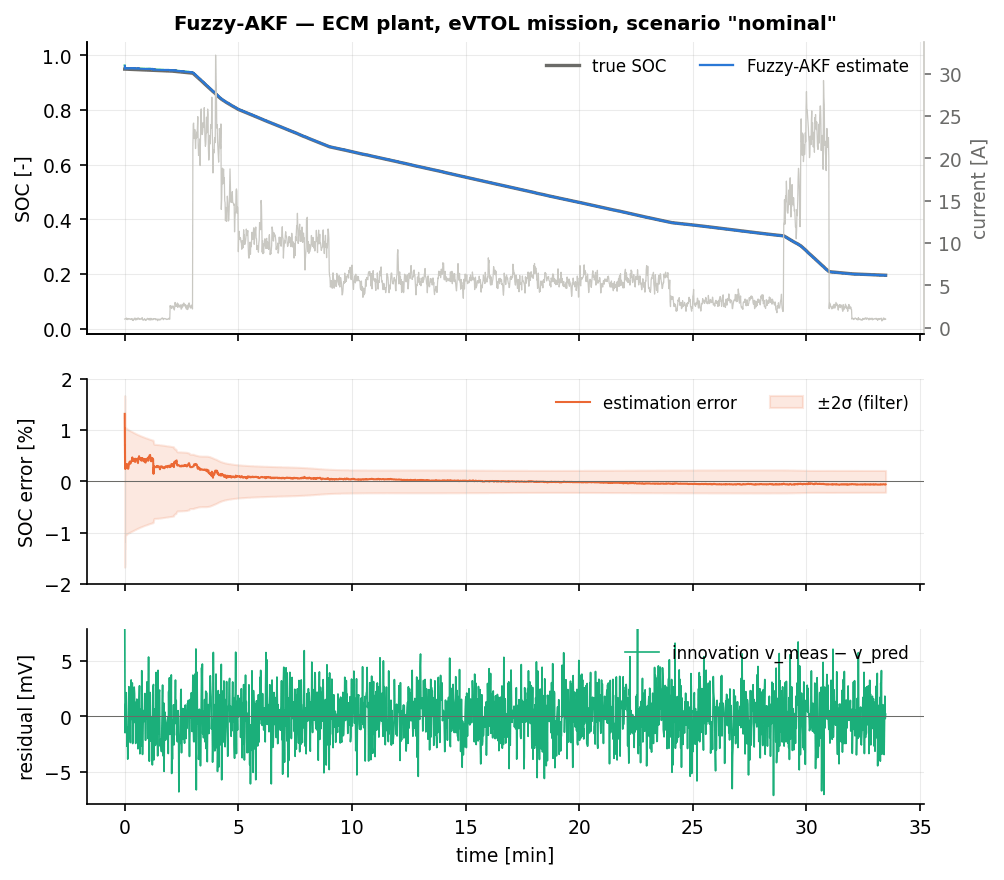
\includegraphics[width=\textwidth]{figures/cell_FuzzyAKF_nominal.png}
\caption{Fuzzy-AKF on the nominal eVTOL mission: true and estimated SOC (top), estimation error with the $\pm 2\sigma$ band when available (middle), voltage residual (bottom).}
\end{figure}
\begin{figure}[H]\centering
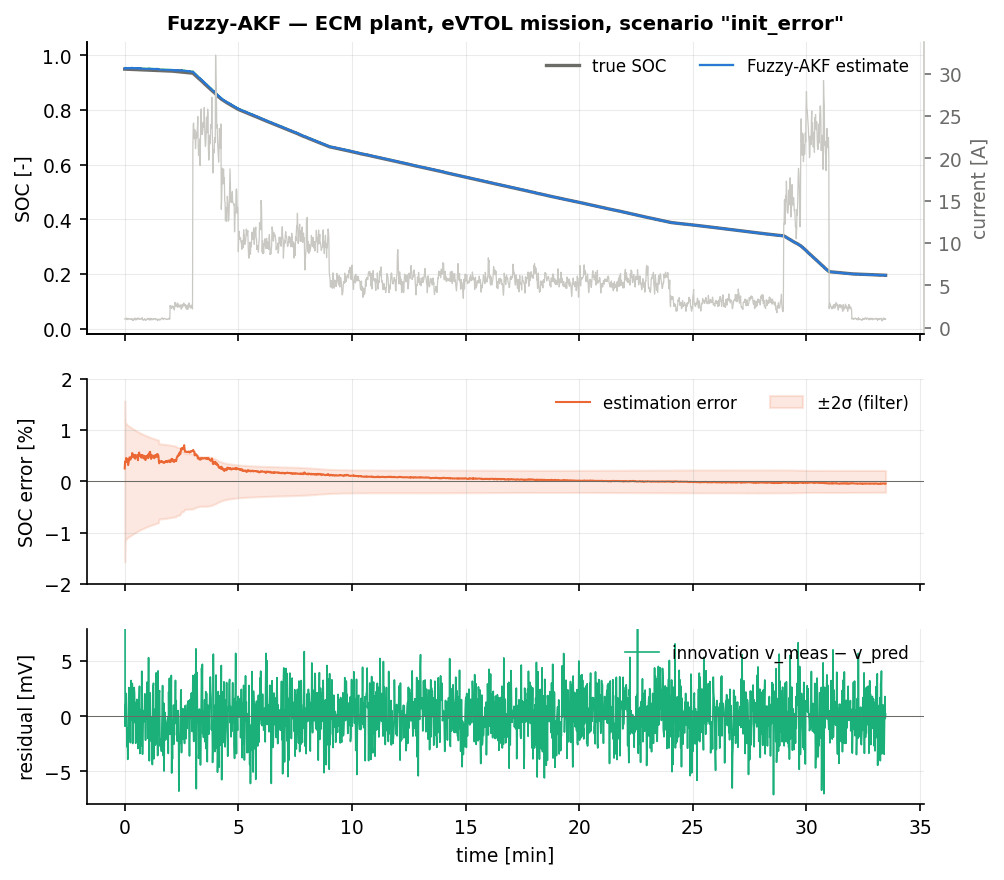
\includegraphics[width=\textwidth]{figures/cell_FuzzyAKF_init_error.png}
\caption{Fuzzy-AKF with a 35\,\% initial SOC error.}
\end{figure}
\begin{figure}[H]\centering
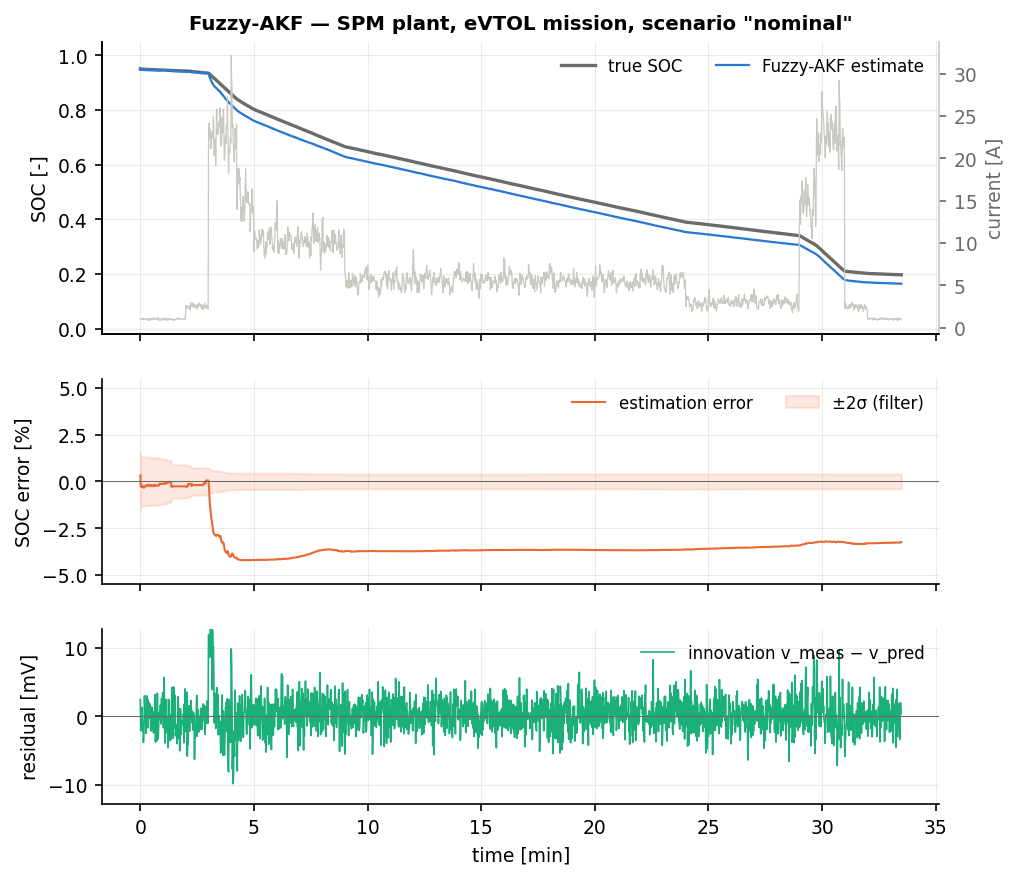
\includegraphics[width=\textwidth]{figures/cellspm_FuzzyAKF_nominal.png}
\caption{Fuzzy-AKF on the electrochemical (single-particle) plant, nominal mission: the estimator uses a 2-RC ECM fitted to that plant and therefore sees a structured \SI{4}{\milli\volt} residual instead of white noise.}
\end{figure}

All figures below are three-seed means in \% SOC, as tabulated above; the plain \texttt{EKF} run on
the same data is the reference (\texttt{EKF ref.} column).  For orientation, the EKF scores
$\mathrm{rmse}_{ss}$ = 0.05\,\% on \texttt{nominal}, 0.12\,\% on \texttt{noise\_step}, 0.21\,\% on
\texttt{outliers}, 0.46\,\% on \texttt{sensor\_dropout}, 1.36\,\% on \texttt{param\_mismatch},
1.52\,\% on \texttt{aged\_cell} and 12.44\,\% on \texttt{combined} (where it never converges), and
3.73\,\% on the nominal SPM mission.

\paragraph{Benign scenarios.}  \texttt{nominal}: $\mathrm{rmse}=0.19\,\%$,
$\mathrm{rmse}_{ss}=0.05\,\%$ against the EKF's $0.15\,\%$ / $0.05\,\%$; the supervisor settles at
$s\approx1.10$, i.e.\ it detects (correctly) that the true innovation energy is about $10\,\%$ above
the nominal model value, mostly because of the ADC quantisation the model does not represent.
\texttt{init\_error}: $0.16\,\%$ / $0.08\,\%$, converging at $t=\SI{0}{\second}$ with a maximum error
of $0.71\,\%$.  Both well inside the $2\,\%$ bound.

\paragraph{Target scenario \texttt{noise\_step}.}  Averaged over $t\in[100,600)\,\si{\second}$ on
seed 1 the scaling is $s=1.10$; over $t\in[700,2010]\,\si{\second}$ it is $s=93.3$, i.e.\
$\hat\sigma_v=\sqrt{93.3}\times\SI{2.09}{\milli\volt}=\SI{20.2}{\milli\volt}$ against the true
\SI{20}{\milli\volt} --- a $1\,\%$ error in the identified standard deviation.  The three-seed SOC
metrics confirm that this is worth having: the EKF's steady-state error rises from $0.05\,\%$ on
\texttt{nominal} to $0.12\,\%$ here, while Fuzzy-AKF holds $\mathbf{0.05\,\%}$, a $2.4\times$
reduction.  The mean normalised innovation squared is $1.019$ before and $1.020$ after the step,
versus $1.099$ and $\mathbf{90.3}$ for the EKF: consistency is fully restored.  The
voltage-prediction error falls from \SI{2.89}{\milli\volt} to \SI{1.02}{\milli\volt}.

\paragraph{Target scenario \texttt{outliers}.}  With $5\,\%$ of samples corrupted by
$\pm\SI{50}{\milli\volt}$ the supervisor settles at $s=31.0$
($\hat\sigma_v=\SI{11.6}{\milli\volt}$, the standard deviation of the contaminated distribution) and
gives $\mathrm{rmse}=0.25\,\%$, $\mathrm{rmse}_{ss}=\mathbf{0.05\,\%}$ against the EKF's $0.52\,\%$ /
$0.21\,\%$ --- a $2.1\times$ reduction of the full-run RMSE and $4.2\times$ in steady state, tying
the variational filter of \cref{ch:vbakf} on the steady-state metric (though VB is twice as good over
the full run, $0.12\,\%$, because it rejects each spike as it arrives).  The rate limit is both the
strength and the weakness here: it prevents the supervisor from being yanked around by the spikes ---
the mean NIS of $2.03$ shows that the filter deliberately does \emph{not} inflate $\mR$ enough to
absorb the outliers into its consistency statistic --- but it also means each individual outlier is
processed with a gain that is only moderately reduced, and the maximum error stays at $2.50\,\%$
against VB's $1.60\,\%$.

\paragraph{Model mismatch.}  \texttt{param\_mismatch}: $\mathrm{rmse}$ $1.28\to0.83\,\%$ and
$\mathrm{rmse}_{ss}$ $1.36\to0.96\,\%$.  \texttt{sensor\_dropout}: $0.72\to0.19\,\%$,
$0.46\to0.06\,\%$ ($3.8\times$ / $7.7\times$, second only to IAE).  \texttt{aged\_cell}:
$1.18\to1.04\,\%$, $1.52\to1.25\,\%$.  \texttt{combined}: the EKF never converges
($t_\mathrm{conv}=$ --, $16.02\,\%$ / $12.44\,\%$); Fuzzy-AKF converges at $t=\SI{1753}{\second}$
with $5.67\,\%$ / $2.56\,\%$, a $2.8\times$ / $4.9\times$ improvement but the slowest convergence and
the weakest steady-state figure of the four $\mR$-adapting filters --- which is the rate limit showing
up exactly where the theory says it will, since the scenario demands a factor-of-sixty change in $s$
from the first sample onwards.  \texttt{preisach} (Preisach hysteresis with the corrected sign
convention in the truth plant) is a draw with the EKF in steady state ($0.20\,\%$ for both, full-run
$0.61\,\%$ against $0.58\,\%$) but converges immediately against the EKF's \SI{16}{\second};
\texttt{cold} ($0.20\,\%$ against $0.16\,\%$) and \texttt{current\_bias} ($0.64\,\%$ against
$0.61\,\%$) are marginally worse, the latter necessarily so, since an input-side error does not show
up in the innovation covariance.

\paragraph{Cost.}  \SI{727}{\nano\second}/step against the EKF's \SI{478}{\nano\second}/step, behind
only VB-AKF and the two multiple-model estimators; the Mamdani centroid grid is $\approx40\,\%$ of the
overhead.

\paragraph{Electrochemical (SPM) plant.}  On the single-particle plant the 2-RC ECM leaves a
structured, slowly varying \SI{4}{\milli\volt} residual, and the fuzzy supervisor reads it exactly as
its rule base instructs: $\tr\hat{\mC}_k$ exceeds $\tr\mS_k$, $\mathrm{DoM}_k$ is firmly positive,
rule $\mathsf{R}_3$ fires at full strength, and $s$ ramps up until the two match.  The result is
$\mathrm{rmse}_{ss}=3.18\,\%$ on the nominal SPM mission against the EKF's $3.73\,\%$, a $15\,\%$
improvement --- essentially identical to the other $\mR$-adapting filters (IAE $3.02\,\%$, VB
$3.18\,\%$, Sage--Husa $3.33\,\%$) and an order of magnitude behind the covariance-inflating ones
(Fading-EKF $0.36\,\%$, STF $0.66\,\%$).  The fixed-point identity \eqref{eq:fz:fp} explains why the
whole $\mR$-adapting group lands in the same place: they all converge to the same covariance-matching
solution, and that solution is the wrong one here.  Matching the innovation covariance means
declaring the voltage channel noisy and reducing the gain, which hands SOC to the coulomb integrator
--- and on the SPM plant the integrator is the faulty part, because the fitted capacity and coulombic
efficiency do not reproduce the true lithium inventory.  The measurement is the trustworthy part: the
ECM's $\ocv(\soc)$ map was fitted to this plant.  Under structured model error the correct move is to
shorten the filter's memory so recent measurements outweigh the accumulated model --- inflating $\mP$
--- and covariance matching does the exact opposite.  Where the SPM scenario adds a second error on
top, the supervisor earns its keep: \texttt{cold} $7.35\to3.09\,\%$ ($2.4\times$),
\texttt{param\_mismatch} $3.13\to1.99\,\%$, \texttt{sensor\_dropout} $5.31\to3.36\,\%$ and
\texttt{current\_bias} $5.69\to5.16\,\%$.  SPM \texttt{outliers} ($2.70\,\%$ against $1.99\,\%$) is
the only regression, and it is the mildest of the four $\mR$-adapting filters --- the rate limit that
costs convergence speed on \texttt{combined} is what protects it here.

\section{Summary}
A three-rule Mamdani supervisor driven by the normalised covariance mismatch is a rate-limited
implementation of innovation-based adaptive estimation, with the same fixed point and a slew rate
the designer chooses explicitly.  Use it when the tuning must change smoothly and explainably --- it
identifies a tenfold voltage-noise step to within $1\,\%$, restores $\overline{\mathrm{NIS}}\approx1$
where the EKF reaches $90$, cuts the steady-state error on \texttt{param\_mismatch}
by $1.4\times$, on \texttt{sensor\_dropout} by $7.7\times$ and on \texttt{outliers} by $4.2\times$.  Do not use it where a fast per-sample reaction is required: on
impulsive noise the variational filter of \cref{ch:vbakf} is twice as good over the full run, and on a large,
sudden model mismatch the rate limit costs several hundred seconds of convergence time.  Its real
attraction is not accuracy but transparency: every element of the mapping from residual to tuning
can be written on one slide and defended to a certification authority.  Like every filter built on
the covariance-matching fixed point \eqref{eq:fz:fp}, it cannot help when the residual is structured
model error: on the electrochemical plant it gains $15\,\%$ on the EKF where a fading-memory filter
gains a factor of ten.
